\section{Simulation environment}
\label{sec:simulator}

To evaluate the performance of a tracker implementation, ground truth is needed. Ground truth cannot be used for measurements directly, so a simulator is also needed. This chapter covers the development of a measurement simulator using historical AIS-data as ground truth. The simulator supports non-regular time interpolation, represents measurements as N-vectors and generates uniform clutter. Three measurement models have been developed (\autoref{sec:sim-sensors}), but only a position measurement with homogeneous variance have been tested in this project. The simulator can be seeded for reproducibility. 
\medskip

\autoref{sec:sim-overview} is an overview of the simulator and covers how it generates measurements and clutter from historical AIS data. \autoref{sec:sim-truth} covers the dataset used in the project and \autoref{sec:sim-sensors} covers the sensor models developed. \autoref{sec:clutter_sphere} then goes into detail of how uniform clutter can be generated on a spherical cap.

% =====================================================================
\subsection{Overview}
\label{sec:sim-overview}

The following section is an overview of the simulator workflow. It takes downloaded historical AIS data and outputs a sequence of measurements, including clutter. This is illustrated in \autoref{fig:simulator_overview}, which demonstrates the flow using a simple example.

\begin{figure}[htbp]
    \centering
    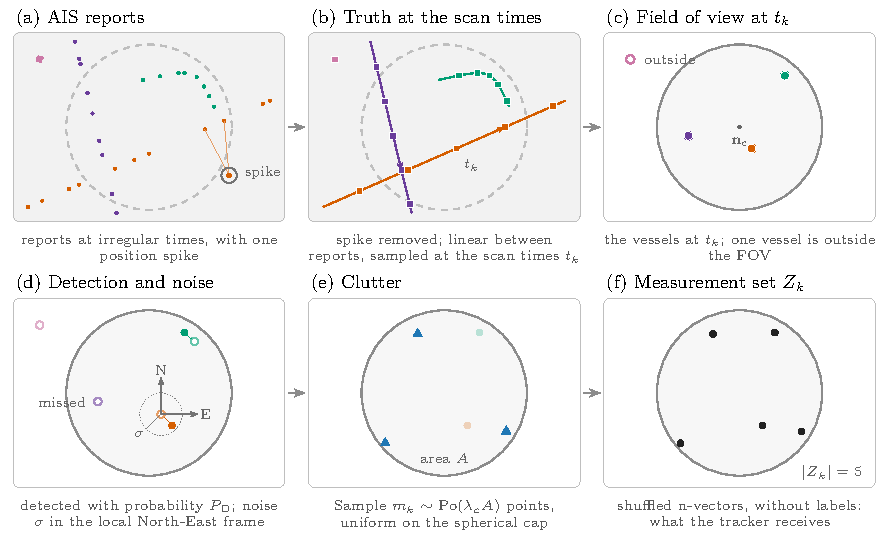
\includegraphics[width=\textwidth]{Images/fig2_storyboard.pdf}
    \caption{Overview of the simulator flow using a simple toy example. Gray panels signal operations that are done once per scenario, while white panels are done for every timestep $t_k$.}
    \label{fig:simulator_overview}
\end{figure}

Part $(a)$ and $(b)$ in \autoref{fig:simulator_overview} is the generation of ground truth for a given scenario. It consists of first cropping AIS from the entire Norwegian waters to the area of interest, then removing outliers. The outlier removal is simple, just consisting of removing points which would result in velocities greater than $30 m/s$. The cleanup removes the worst noise and enables velocity to be returned alongside position. After cropping and outlier removal, points are linearly interpolated between. Velocity is assumed constant and found by dividing distance between points by time between the reports. Positions and velocities are then sampled at arbitrary intervals and returned for all vessels in the area of interest. Positions are N-vectors while velocities are defined in the local North-East frame
\medskip

Looking back at the rest of \autoref{fig:simulator_overview}, we do the following for each set of sampled points at $t_k$. $(c)$, Vessels outside the sensor field of view are dropped. They cannot generate measurements at this time. $(d)$, each vessel within the FOV generates a measurement with probability $\PD$. If a vessel generates a measurement it is Gaussian in the local North-East frame with variance $\sigma$. $(e)$, uniform clutter is generated within the FOV. The number of clutter points is governed by the FOV area and the clutter intensity. The points are generated in such a way that they are uniform on the sphere, see \autoref{sec:clutter_sphere}. $(f)$, measurements and clutter are shuffled by the simulator such that the tracker does not know which measurements are from vessels. The final output is then a set of N-vectors, corresponding to measurements, for each timestep $t_k$.

% =====================================================================
\subsection{Ground truth from AIS}
\label{sec:sim-truth}

The data used as ground truth is historical AIS. It is downloaded from Kystverkets historical AIS database \cite{kystverket}. Minimal filtering is applied to the data, meaning it is not specifically curated for tracking. A consequence is then that the data includes a lot of stationary vessels. In scenarios centered around big ports, around 80\,\% of vessels can be stationary, leading to a realistic, but perhaps unusual scenario in terms of tracking literature. These vessels are usually also quite close in proximity, making association difficult in noisy environments. 

% =====================================================================
\subsection{Sensor models}
\label{sec:sim-sensors}

Three relevant sensor models were developed for the simulator: EO, SAR and NRD. As per the problem formulation, all sensors have abstracted away the detector, leaving three sensors measuring position. The difference between the sensors then lie in the noise and clutter assumptions of the models. EO is modelled as having constant noise, while SAR noise increases with target velocity and NRD noise with distance from the measurement center. For simplicity, only EO is used when evaluating tracker performance. Nonetheless, all models and their modelling assumptions are listed in the subsections below.
\medskip

All sensors are also modelled to have spherical field of views. This is done simply because of N-vector geometry. The field of view is defined by an N-vector center and a radius. Determining which targets are inside or outside the FOV is then simply a dot product between N-vectors.

\subsubsection{Electro-optical (EO) measurements}
As with both SAR and NRD, Electro-optical detectors are complicated and best abstracted away. Again, we are left with a direct position measurement on the form:

\[
z = Hx + v, \quad H = \begin{bmatrix} I & 0 \end{bmatrix}
\]
With the noise $v$ is defined as
\[
v \sim \mathcal{N}(\mathbf{0}, \mathbf{R})
\]
Where $\mathbf{R}$ is the measurement noise covariance matrix. In the case of EO, the variance is not reported by the sensor, thus we model all measurements with the same covariance matrix $\mathbf{R}$.

\subsubsection{Synthetic Aperture Radar (SAR)}
SAR is a type of radar that can be affixed to either satellites or aircraft, moving above the earths surface. There is a lot that can be said about SAR and detecting objects using it. The detection algorithms can be very complex beasts and there is a whole field of research dedicated to just detecting objects using SAR. Here however, we will be using very simple models for the detections. We abstract away the detector entirely and assume only position is retuned. The detector will also return a possibly empty set of false detections. This means that a clutter model should also be included when updating states from a SAR measurement.
\medskip

A standard assumption for SAR detectors is that objects are stationary. When this assumption is invalidated, phenomena such as SAR azimuth shift can occur. SAR azimuth shift occurs when an object has a velocity component that is perpendicular to the radar platform velocity vector \cite{SAR_azimuth_shift}. The geometry and result can be seen in \autoref{fig:sar_azimuth_shift}, where the imaged position is shifted in relation to the true position.

\begin{figure}[htp]
    \centering
    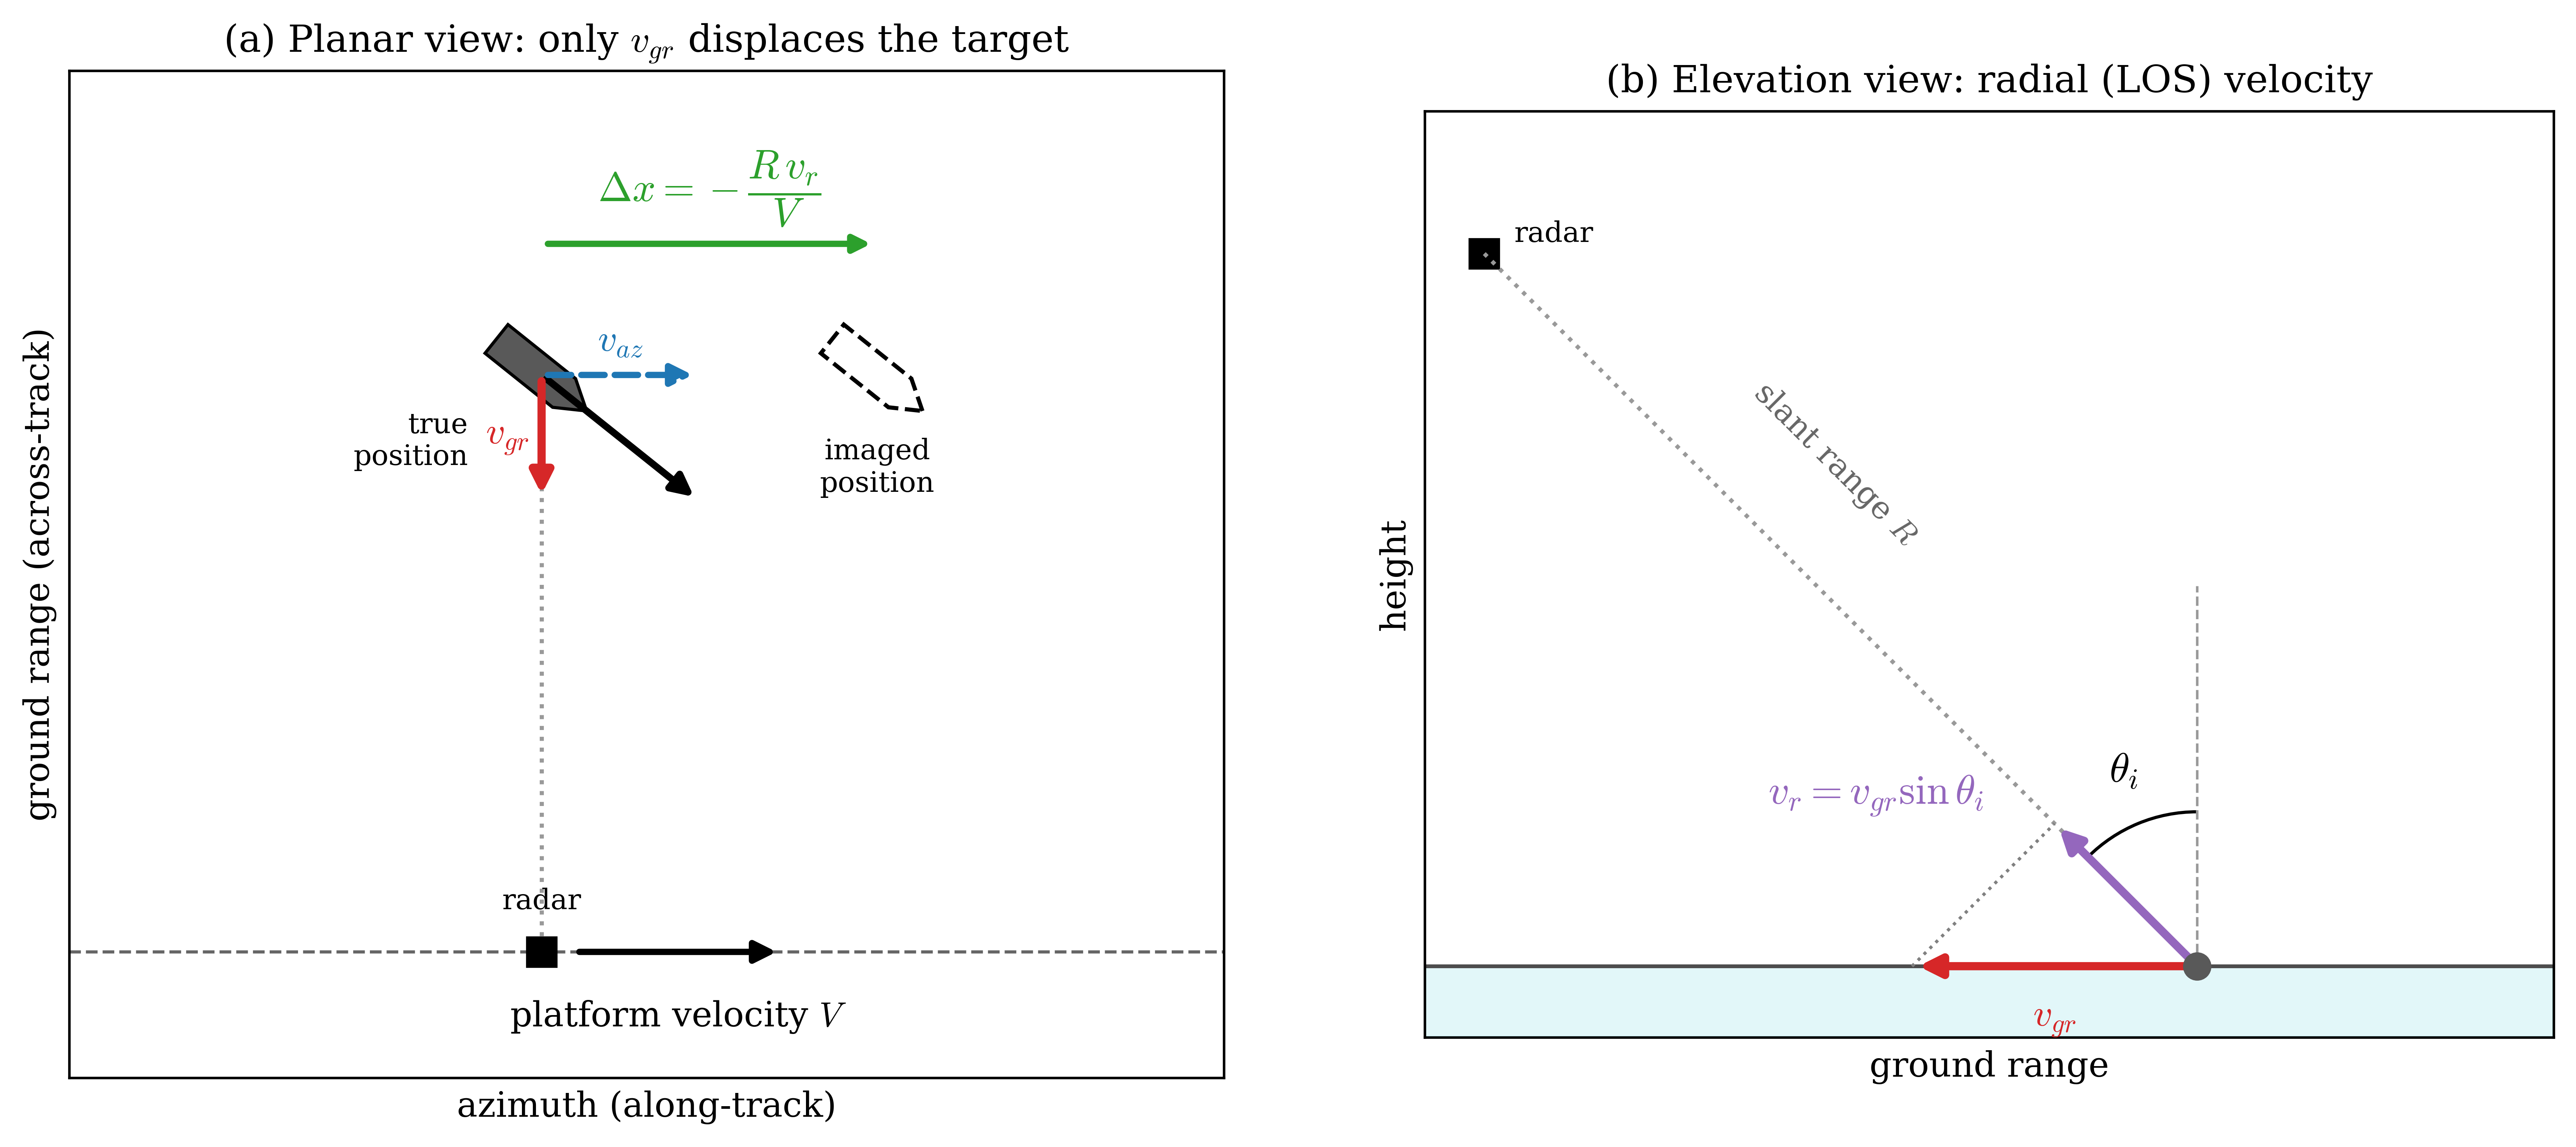
\includegraphics[width=0.95\textwidth]{Images/sar_azimuth_shift.png}
    \caption{Depicting the geometry of SAR azimuth shift. Subfigure $(a)$ shows the decomposed target velocity vector alongside the velocity vector of the radar platform. Subfigure $(b)$ shows the projected velocity component into the line of sight. This is the component that causes the Doppler offset.}
    \label{fig:sar_azimuth_shift}
\end{figure}

Since the azimuth shift is a known deterministic phenomenon, it can be compensated for. The main difficulty regarding compensation is that the velocity vector of the moving target must be known. This is fine for simulating measurements, but robust estimation of velocity in a multi target tracking scenario may be infeasible. It may also be unwanted, since using estimated states to compensate the measurement ruins the linear assumptions of the filtering, and may cause unforeseen consequences.
\medskip

There are two other ways one could incorporate azimuth shift in the measurement model. One alternative is to increase the noise of each measurement based on the absolute velocity of each vessel. It is generally easier to get a good estimate of how fast something is moving than to estimate the direction as well. This yields the measurement model below and may yield better results than estimating the exact azimuth shift. It does however also invalidate the linear assumptions of the filter and needs to be tested rigorously in various conditions.
\[
z = Hx + v(\nu), \quad H = \begin{bmatrix} I & 0 \end{bmatrix}
\]
With the noise $v(\nu)$ is defined as
\[
v(\nu) \sim \mathcal{N}(\mathbf{0}, \mathbf{R}(\nu))
\]
Where $\mathbf{R}$ is the measurement noise covariance matrix.
\medskip

The last approach is to just increase the measurement noise, but keep it constant for all measurements. This keeps the filter linear and is in many ways the ``safest'', but it will reduce the value of measurements where the vessel is at low velocity.

\subsubsection{Navigation Radar Detector (NRD)}
NRD is a satellite borne detector, which tracks and locates the radar signals from civilian navigation radars \cite{nrd_ffi}. For tracking this means that the detector can be abstracted away, leaving a pure position measurement. What is special about NRD is that it can report the uncertainty of the measurement alongside each measurement. This means $R$ can be individual to each measurement. In general, the uncertainty increases radially around the center point of our measurement. This is useful for both simulation and filtering since the uncertainty is dependent on the measurement position and not the state position. One strength with NRD is that since it only detects radar signals, false positives are almost non-existent. This means that the measurements can be assumed to have a clutter intensity of almost zero. The measurement model, stated for completeness is then:

\[
z_i = Hx + v_i, \quad H = \begin{bmatrix} I & 0 \end{bmatrix}
\]
With the noise $v_i$ is defined as
\[
v_i \sim \mathcal{N}(\mathbf{0}, \mathbf{R}_i)
\]
Where $\mathbf{R}_i$ is the measurement noise covariance matrix, which is individual to each measurement.


% =====================================================================
\subsection{Clutter on a sphere}
\label{sec:clutter_sphere}

A standard clutter model used for target tracking is the uniform Poisson clutter model. It is parameterized by the clutter intensity $\lambda_c$, which is the expected number of clutter measurements per unit area/volume. Each clutter measurement is independent, and uniformly distributed within the measurement area. In a rectangular measurement area the generation of a clutter measurement is trivial.

\begin{equation*}
    x = \mathcal{U}(\text{min}_x, \text{max}_x) \quad y = \mathcal{U}(\text{min}_y, \text{max}_y)
\end{equation*}

We would now like to sample uniform clutter on the surface of a sphere, the measurement area defined by a maximum angle $\theta_{max}$ between N-vectors of the center and the measurement rim. This is the same approach used earlier for gating. An illustration of the uniform clutter can be seen in \autoref{fig:spherical_cap}.

\begin{figure}[htp]
    \centering
    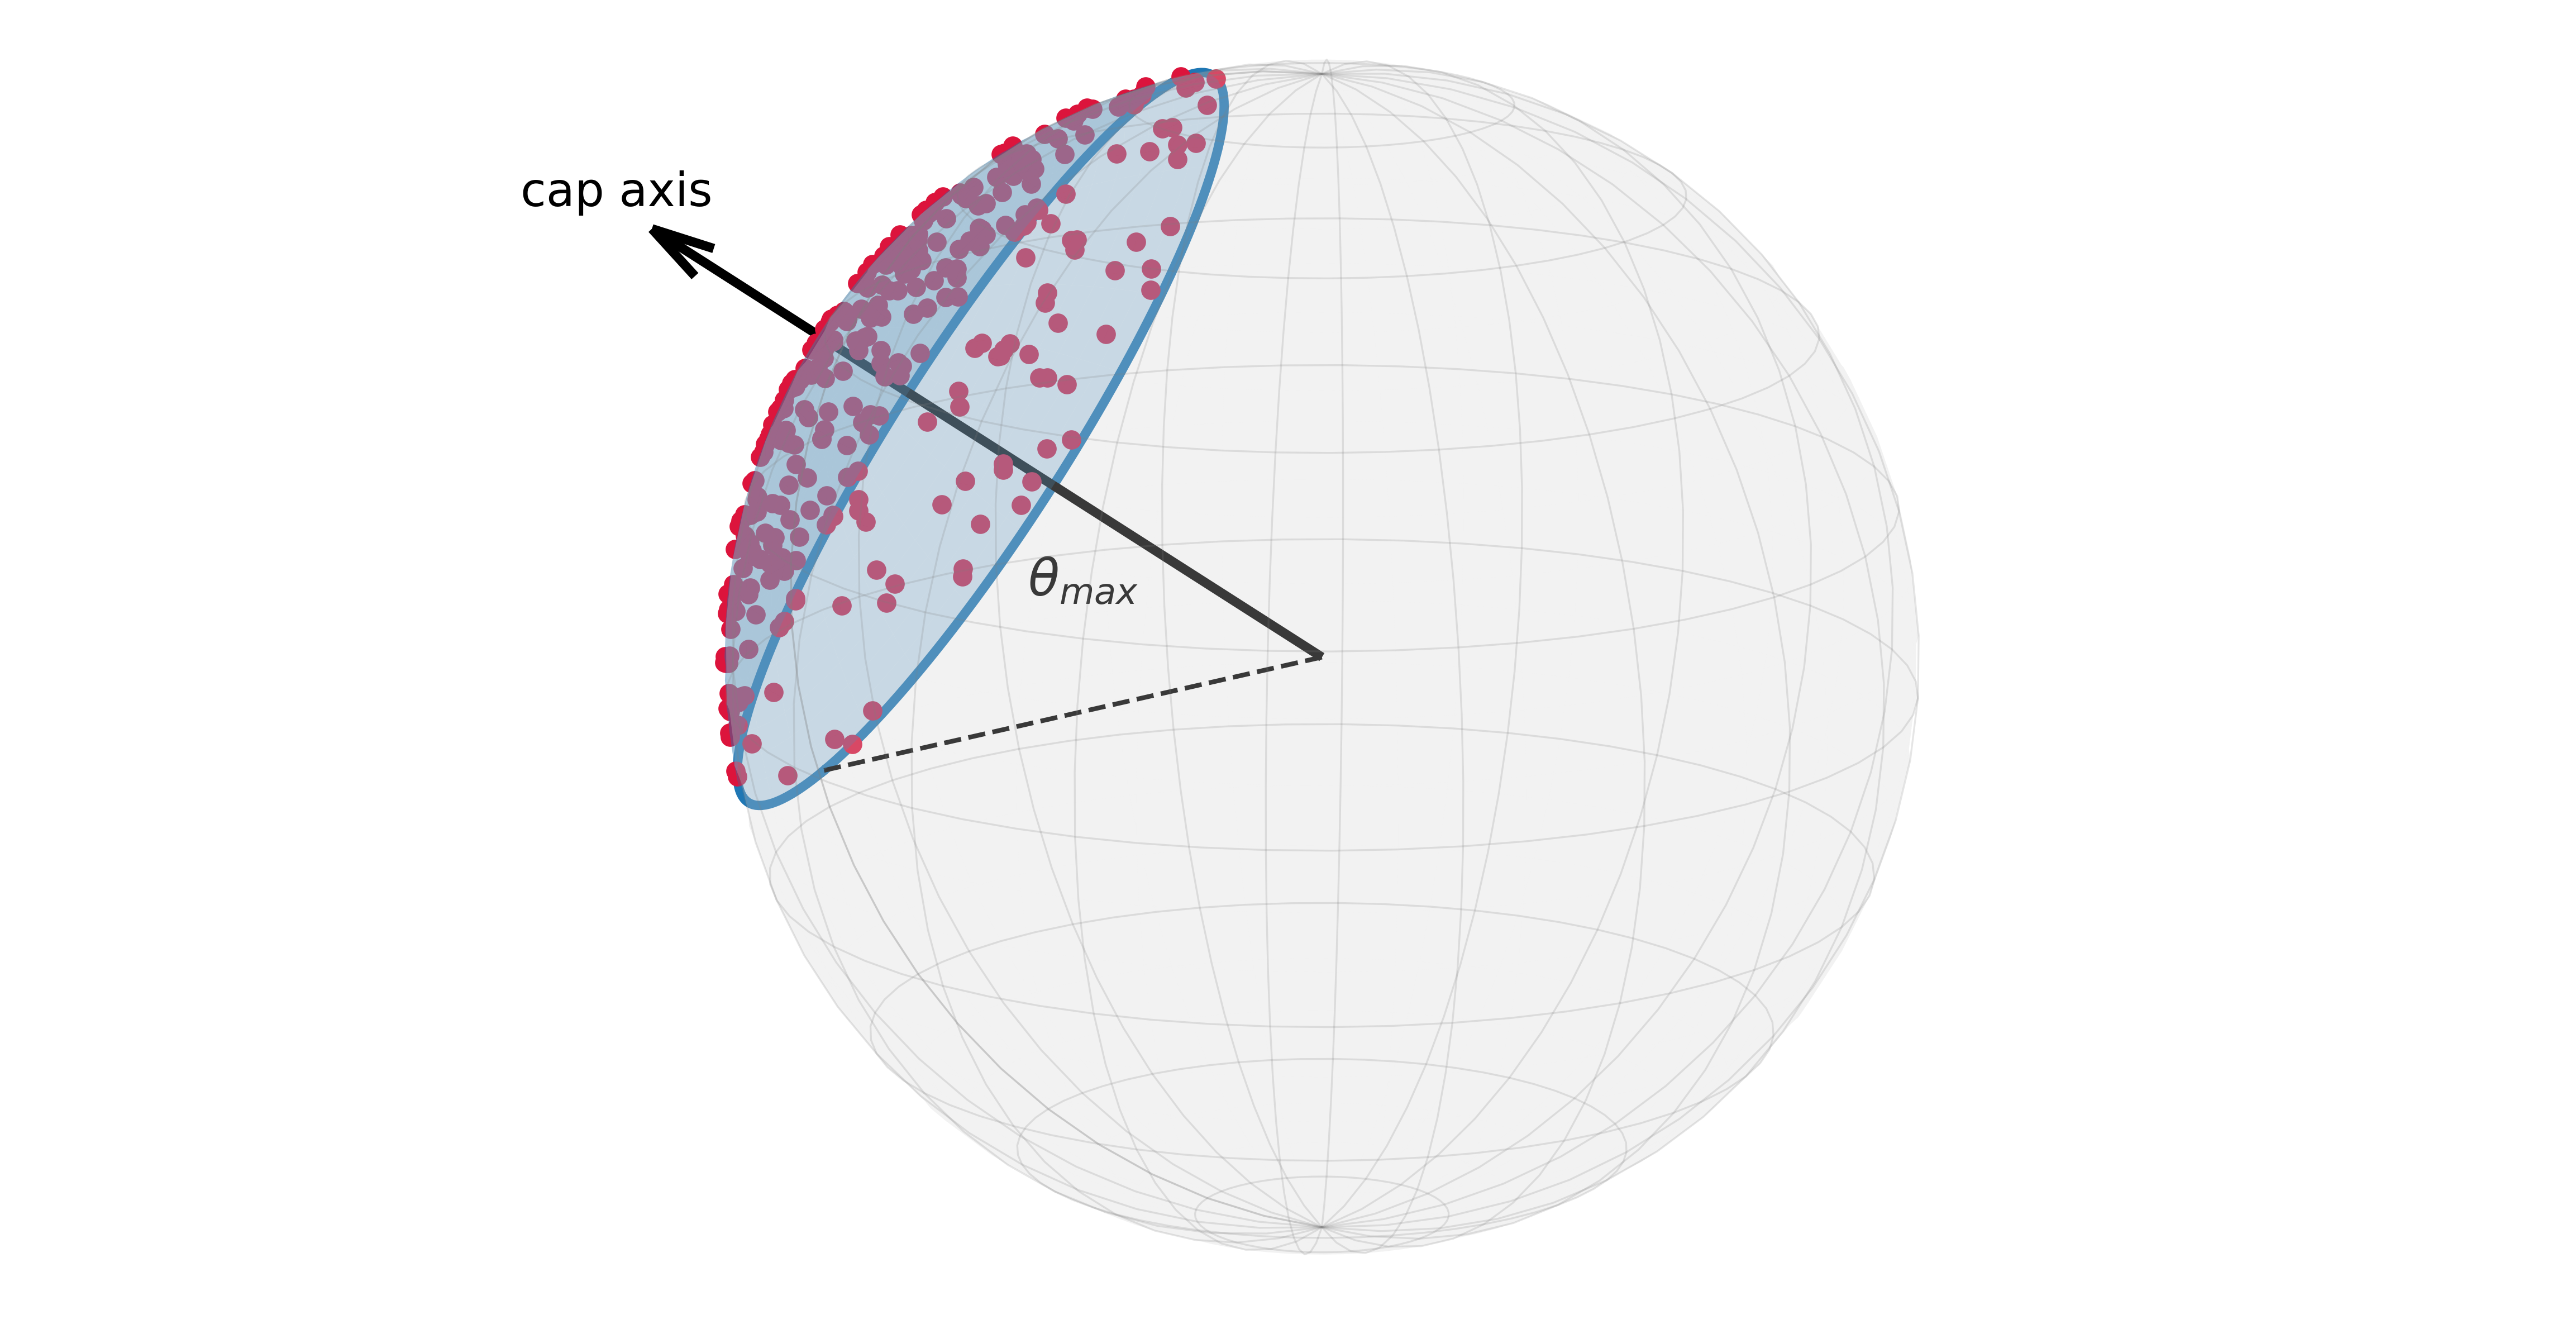
\includegraphics[width=0.8\textwidth]{Images/spherical_cap.png}
    \caption{Points sampled uniformly on a spherical cap, centered around an arbitrary axis.}
    \label{fig:spherical_cap}
\end{figure}

The first part of sampling clutter is to sample the number of clutter measurements, or the cardinality of the Poisson point process if you want. We denote this number $m_k$ and sample it from a Poisson distribution $m_k \sim \text{Po}(\lambda_c A)$. The surface area $A$ of a spherical cap, can be parameterized a few different ways, but using $R$ as the radius of the sphere and $\theta_{max}$ is the most natural in this case. The area is then given by the following formula \parencite{spherical_cap}.

\begin{equation*}
    A = 2 \pi R^2 (1 - \cos(\theta_{max}))
\end{equation*}

The clutter measurements should then be uniformly distributed on the spherical cap. The derivation is explained in detail in \parencite{clutter_sphere}, so I will only touch over the main points here. 
\medskip

We can parameterize the points on the spherical cap by the cap axis (N-vector), radial distance from the cap axis ($\theta \in [0, \theta_{max}]$) and angle between the point and some arbitrary reference point ($\psi \in [0, 2 \pi]$). The angle $\psi$ is illustrated in \autoref{fig:psi_illustration}. We can then sample two independent uniform distributions and get uniform points on the spherical cap by the following transformations.

\begin{figure}[htp]
    \centering
    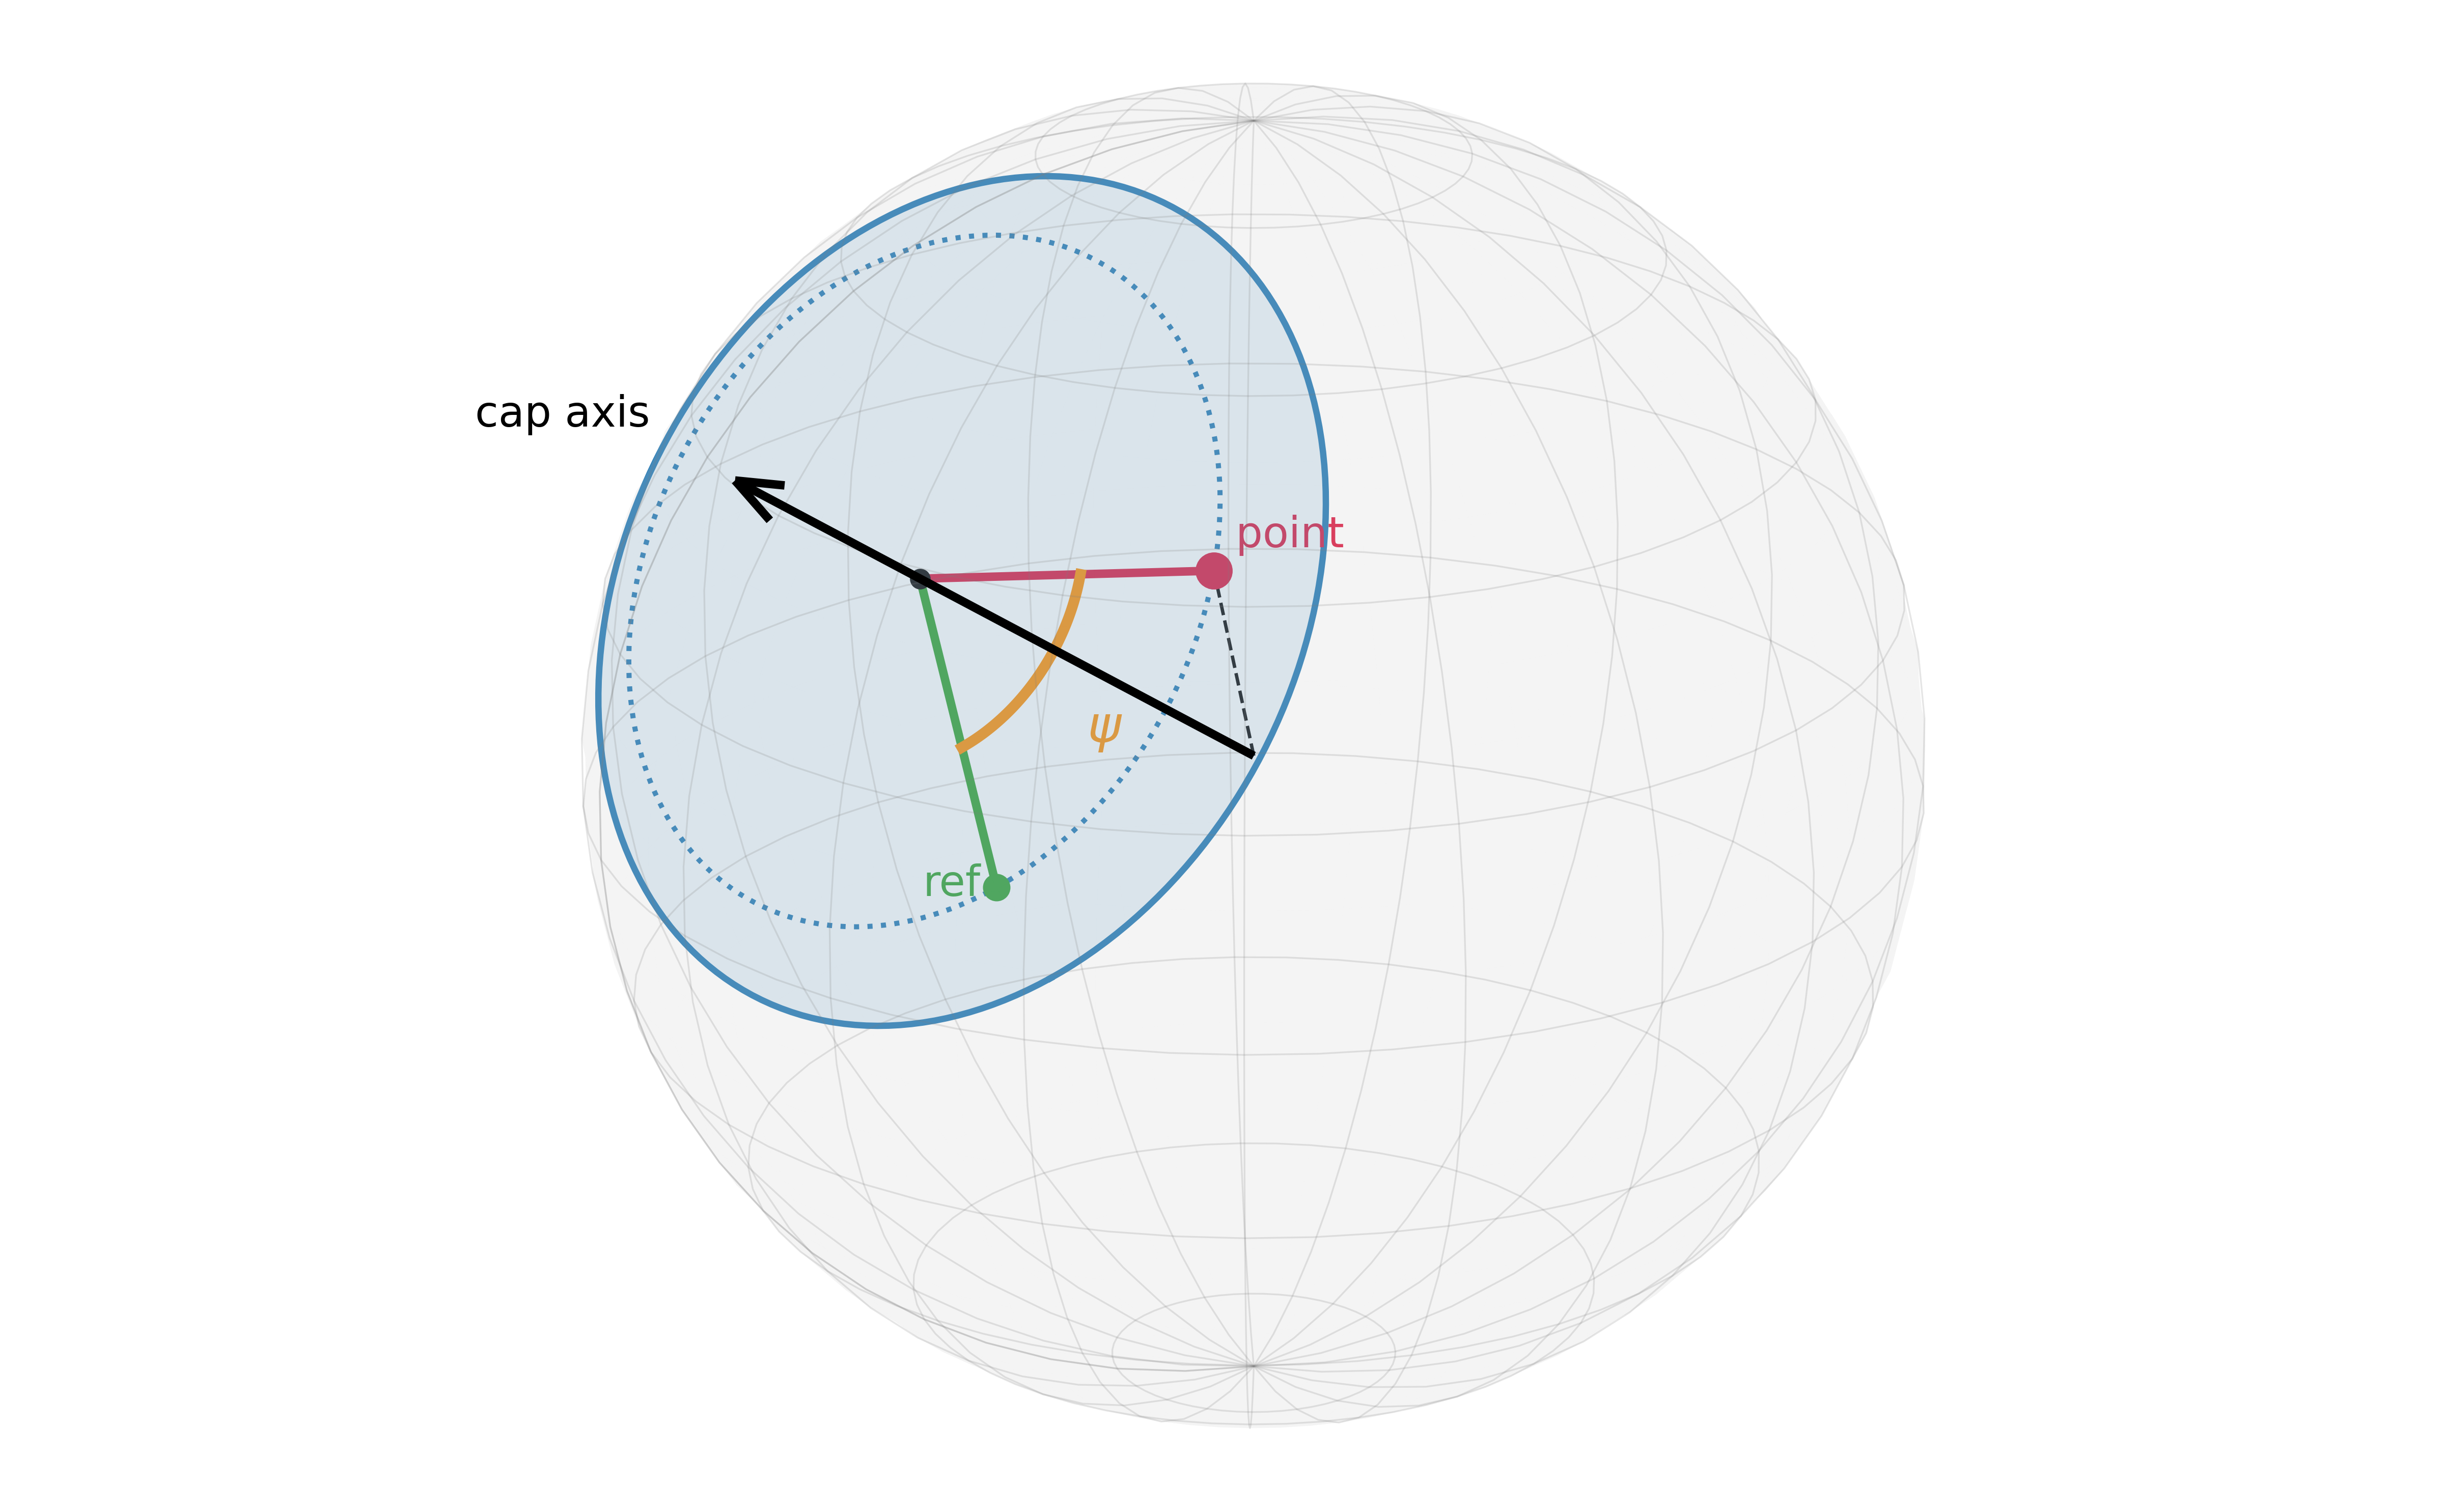
\includegraphics[width=0.8\textwidth]{Images/psi_illustration.png}
    \caption{An illustration of the angle $\psi$}
    \label{fig:psi_illustration}
\end{figure}

\begin{equation*}
    U_1 = \mathcal{U}(0, 1) \quad U_2 = \mathcal{U}(0, 2 \pi)
\end{equation*}

\begin{align*}
    \psi &= U_2 \\
    z &= \cos(\theta_{max}) + U_1 (1-\cos(\theta_{max})) \\
    \theta &= \cos^{-1}(z)
\end{align*}

The uniform point can then be returned as an N-vector by following Example 8 in \parencite{ffi_nvector}. Note that since the points sampled are random and uniform, the result is invariant to rotation about the cap axis. This means that it is not necessary to specify $\psi$ and $\theta$ in the correct East - North frame.

% =====================================================================
%\subsection{Scenarios}
%\label{sec:sim-scenarios}
%\begin{itemize}
%    \item One table of the windows used, with centre, radius, start, scans, scan interval, vessels in view and share moving.
%    \item Proof-of-concept window: 59.09$^\circ$\,N, 5.45$^\circ$\,E, radius 12~km, 60 scans of 60~s, 14--19 vessels.
%    \item Scale windows: same centre, radius 12--100~km, 30 scans, 17--398 vessels.
%    \item Named scenarios on the national data (fjords, open water, shipping lanes), and how they were selected (enough vessels, no long AIS gaps for moving vessels). Use only the ones the results use.
%    \item One map figure of a scenario with truth and measurements.
%\end{itemize}
